\documentclass[12pt, a4paper]{report}

\usepackage{libertine}
\usepackage{libertinust1math}
\usepackage{inconsolata}
\usepackage{amsthm, amsmath}
\usepackage[style=german]{csquotes}
\usepackage[pagestyles]{titlesec}
\usepackage[romanian]{babel}
\usepackage{tikz}
\usetikzlibrary{er,positioning}
\usepackage{soul}
\usepackage{tocloft}
\usepackage{enumerate}
\usepackage{setspace}
\usepackage{subcaption}
\usepackage{bm}
\usepackage{xcolor}
\usepackage{todonotes}
\usepackage{graphicx}
\usepackage{array}
\usepackage[all]{xy}
\setcounter{MaxMatrixCols}{20}
\usepackage{fancyhdr}
% \usepackage{natbib}     % citekey hyphenation
\usepackage{marginnote}
\usepackage{imakeidx}
\makeindex[options= -s indices-alph.ist]
\usepackage{hyperref}
\hypersetup{citecolor=blue}
\usepackage{fontawesome}

\newcommand\NN{\mathbb{N}}
\newcommand\ZZ{\mathbb{Z}}
\newcommand\QQ{\mathbb{Q}}
\newcommand\RR{\mathbb{R}}
\newcommand\CC{\mathbb{C}}
\newcommand\AF{\mathbb{A}}
\newcommand\PP{\mathbb{P}}
\newcommand\FF{\mathbb{F}}
\newcommand\bb{\mathbb}
\newcommand\dr{\mathrm}
\newcommand\kal{\mathscr}
\newcommand\fk{\mathfrak}
\newcommand\op{\oplus}
\newcommand\ot{\otimes}
\newcommand\ds{\displaystyle}
\newcommand\id{\indent}
\newcommand\nid{\noindent}
\newcommand\seq{\subseteq}
\newcommand\sneq{\subsetneq}
\newcommand\speq{\supseteq}
\newcommand\spneq{\supsetneq}
\newcommand\rar{\rightarrow}
\newcommand\Rar{\Rightarrow}
\newcommand\xrar{\xrightarrow}
\newcommand\lar{\leftarrow}
\newcommand\Lar{\Leftarrow}
\newcommand\xlar{\xleftarrow}
\newcommand\lrar{\leftrightarrow}
\newcommand\Lrar{\Leftrightarrow}
\newcommand\ideal{\trianglelefteq}
\newcommand\such{\text{ s.t. }}
\newcommand\sk{(\textit{Sketch}) }
\newcommand\rhup{\rightharpoonup}
\newcommand\rhdn{\rightharpoondown}
\newcommand\lhup{\leftharpoonup}
\newcommand\lhdn{\leftharpoondown}
\newcommand\incl{\hookrightarrow}
\newcommand\vid{\emptyset}
\newcommand\wt{\widetilde}
\newcommand\wh{\widehat}
\newcommand\ol{\overline}
\newcommand\Lor{\Longrightarrow}
\newcommand\Lol{\Longleftarrow}
\newcommand\Lolr{\Longleftrightarrow}
\newcommand\ld{{}^\ast}
\newcommand\lgr{{}^{\ast-\text{gr}}}
\newcommand\kap{\Bbbk^a[\kal{P}]}
\newcommand\kcp{\Bbbk^c[\kal{P}]}
\newcommand\fc{\mathfrak{c}}
\newcommand\qq{\enquote}
\newcommand\coli{\protect\varinjlim}
\newcommand\li{\protect\varprojlim}
\newcommand\injr{\rightarrowtail}
\newcommand\surjr{\twoheadrightarrow}
\newcommand\injl{\leftarrowtail}
\newcommand\surjl{\twoheadleftarrow}
\newcommand\sqsb{\sqsubseteq}
% THEOREMS
\newtheoremstyle{dotless}{}{}{\itshape}{}{\bfseries}{:}{ }{}
\theoremstyle{dotless}
\newtheorem{theorem}{Teorem\u{a}}[section]
\newtheorem{proposition}{Propozi\c{t}ie}[section]
\newtheorem{lemma}{Lem\u{a}}[section]
\newtheorem{corollary}{Corola}[section]
\newtheorem{axiom}{Axiom\u{a}}[section]
\newtheorem{principle}{Principiu}[section]
\newtheorem{reg}{Regul\u{a}}[section]
\renewcommand*{\proofname}{Dem.:}

\newtheoremstyle{dotlessdr}{}{}{}{}{\bfseries}{:}{ }{}
\theoremstyle{dotlessdr}
\newtheorem{example}{Exemplu}[section]
\newtheorem{definition}{Defini\c{t}ie}[section]
\newtheorem{remark}{Observa\c{t}ie}[section]
\newtheorem{exercise}{Exerci\c{t}iu}[section]
\numberwithin{equation}{section}
% FONTS
\usepackage[mathscr]{euscript}
\usepackage[normalem]{ulem}
\usepackage{eurosym}
\usepackage{sectsty}
\allsectionsfont{\rmfamily}
\usepackage{anyfontsize}

% PAGE SETUP
\usepackage[portrait]{geometry}
\geometry{
  a4paper,
  left=20mm,
  right=25mm,
  % marginparwidth=40mm,
}
\usepackage{afterpage}
\newcommand\blankpage{
  \null
  \thispagestyle{empty}
  \addtocounter{page}{-1}
  \newpage}
\newenvironment{myenv}[1]
  {\begin{spacing}{#1}}
    {\end{spacing}}

% FANCY SETUP
\usepackage[Glenn]{fncychap}
\usepackage{fancyhdr}
\addto\captionsromanian{\renewcommand{\chaptername}{Secțiunea}}


\begin{document}

\thispagestyle{empty}
\pagestyle{plain} % fix for page numbers

\title{\huge\textbf{Numărul de puncte \\ ale curbelor eliptice}}
\vspace{1cm}
\author{\Large\textsc{Adrian Manea}}

\maketitle

\pagenumbering{gobble}
\tableofcontents

\setcounter{page}{1} % page 1 after TOC

%%%%%%%%%%%%%%%%%%%%%%%%%%%%%%%%%%%%%%%%%%%%%%%%%%
% MAIN CONTENT
\pagenumbering{arabic}
\pagestyle{fancy}
\fancyhf{}
\rhead{\footnotesize{\color{gray}Puncte ale curbelor eliptice}}
\lhead{\footnotesize{\color{gray}Adrian Manea, 510 SLA}}

\pagestyle{plain} % restore page numbering

% DE ADĂUGAT
\addcontentsline{toc}{chapter}{\protect\numberline{}DE ADĂUGAT/CLARIFICAT}
\listoftodos[DE ADĂUGAT/CLARIFICAT]

% CHAPTERS
%! TEX root = ../tamarin.tex

\chapter{Introducere}

% ! TEX root = ../pce.tex

\chapter{Curbe eliptice}

\section{Generalități}

Formal, curbele eliptice sînt varietăți proiective de dimensiune 1 și gen 1,
dar ele pot fi definite și intuitiv, la nivel elementar, folosind forma
dată de așa-numita \emph{ecuație Weierstrass}.

Fără a intra în detalii generale privitoare la funcțiile Weierstrass, este
suficient să definim o \emph{curbă eliptică} printr-o ecuație de forma:
\[
  y^2 = x^3 + ax + b,
\]
care este \emph{nesingulară}, adică nu conține \qq{colțuri} (eng.\ \emph{cusps})
și autointersecții. În funcție de corpul peste care este definită curba
eliptică, coeficienții $ a, b $ sînt elemente ale corpului respectiv.

Clasificarea curbelor eliptice se face folosind \emph{discriminantul} curbei,
care se definește prin:
\[
  \Delta = -16(4a^3 + 27b^2),
\]
care trebuie să fie nenul ca să avem o curbă nesingulară.

Aplicațiile în geometrie algebrică și criptografie sînt facilitate de posibilitatea
definirii unei structuri de grup pe mulțimea punctelor de pe o curbă eliptică.
Această structură de grup este bine precizată riguros, folosind \emph{divizori}
(cf., de exemplu, \cite{sil09}, III.\S2), dar pentru scopurile lucrării prezente
va fi suficient să descriem operația de grup intuitiv.

Astfel, fie $ P $ și $ Q $ două puncte de pe curbă. Putem descrie punctul $ P + Q $
astfel: se trasează dreapta care conține cele două puncte și al treilea punct
de intersecție al acestei drepte cu curba se definește ca fiind opusul rezultatului.

Formal, avem:
\begin{definition}\label{def:adunare-pc}
  Fie $ E $ o curbă eliptică și fie $ P, Q $ două puncte pe $ E $.

  Fie $ L $ dreapta prin $ P $ și $ Q $ (dacă $ P = Q $, atunci $ L $ va
  fi tangenta în $ P $). Fie $ R $ un al treilea punct de intersecție al
  lui $ L $ cu $ E $.

  Fie $ L' $ dreapta care unește $ R $ și $ O = [0, 1, 0] $, punctul de la
  infinit.

  Atunci $ L' $ intersectează $ E $ în $ R, O $ și un al treilea punct,
  care se notează $ P + Q $.
\end{definition}

Operația este ilustrată în figura \ref{fig:pc-adunare}
\begin{figure}[!htbp]
  \centering
  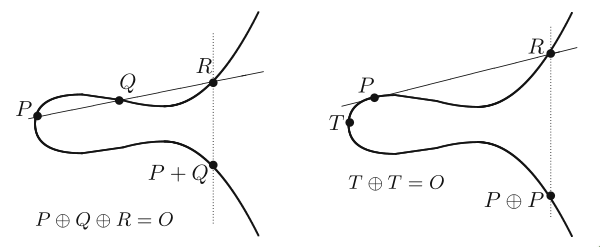
\includegraphics[scale=0.5]{fig/adunare-el.png}
  \caption{\textit{Adunarea punctelor pe o curbă eliptică, \cite{sil09}, p.\ 51}}
  \label{fig:pc-adunare}
\end{figure}

Cu această operație $ (E, +) $ formează un grup abelian, cu elementul neutru
$ O = [0, 1, 0] $.

\begin{example}\label{exm:adunare-pc}
  Fie curba eliptică $ E $, definită peste $ \QQ $ prin ecuația Weierstrass:
  \[
    E : y^2 = x^3 + 17.
  \]
  Calcule simple găsesc cîteva puncte cu coordonate întregi:
  \[
    P_1 = (-2, 3), \quad P_2 = (-1, 4), \quad P_3 = (2, 5), \quad P_4 = (4, 9), %
    \quad P_5 = (8, 23).
  \]
  Folosind operația de grup, putem verifica relațiile:
  \[
    P_5 = -2 \cdot P_1, \quad P_4 = P_1 - P_3.
  \]

  Mai general, de fapt, se poate arăta că orice punct rațional $ P \in E(\QQ) $
  poate fi scris sub forma:
  \[
    P = mP_1 + nP_3, \quad m, n \in \ZZ,
  \]
  de unde rezultă că $ E(\QQ) = \ZZ \times \ZZ $.
\end{example}

%%%%%%%%%%%%%%%%%%%%%%%%%%%%%%%%%%%%%%%%%%%%%%%%%%%%%%%%%%%%%%%%%%%%%%

\section{Aplicația Frobenius}

Lucrăm în cazul particular cînd curba $ E $ este definită peste un corp finit
$ \FF_q $ (caz dezvoltat și în secțiunile următoare). Așadar, considerăm
$ q $ o putere a unui prim $ p $, iar $ \FF_q $ va fi corpul cu $ q $
elemente.

Se definește \emph{aplicația Frobenius} prin:
\[
  \phi : E \to E, \quad \phi(x, y) = (x^q, y^q).
\]

Mai general, dacă $ K $ este un corp care-l extinde pe $ \FF_q $,
se poate defini morfismul Frobenius $ F $ în general prin
$ \alpha \mapsto \alpha^q $.

Cîteva proprietăți elementare, preluate fără demonstrație din \cite{soe}:
\begin{proposition}\label{pr:propr-frob}
  Aplicația $ F : K \to K $ de mai sus satisface proprietățile:
  \begin{enumerate}[(a)]
  \item $ F(xy) = F(x) F(y), \forall x, y \in K $;
  \item $ F(x + y) = F(x) + F(y), \forall x, y \in K $;
  \item $ \FF_q = \{ \alpha \in K \mid F(\alpha) = \alpha \} $;
  \item Dacă $ K = \FF_q(t) $ este corpul de funcții raționale
    peste $ \FF_q $, într-o nedeterminată $ t $, atunci pentru o funcție
    rațională $ \gamma \in \FF_q(t) $ are loc $ F(\gamma(t)) = \gamma(t^q) $.
  \end{enumerate}
\end{proposition}

Demonstrațiile sînt manipulări algebrice simple ale proprietăților corpurilor
finite, precum și ale caracteristicii $ q $, în mod esențial.

De asemenea, aplicația Frobenius este bijectivă.

\todo[inline,noline,backgroundcolor=green!40]{poate ceva despre polinoamele de diviziune?}

%%% Local Variables:
%%% mode: latex
%%% TeX-master: "../pce"
%%% End:

% ! TEX root = ../pce.tex

\chapter{Numărul de puncte peste $ \FF_{\text{q}} $}

\section{Problema și abordarea naivă}

Fie acum $ E/\FF_q $ o curbă eliptică definită peste un corp finit.
Vrem să estimăm numărul punctelor din $ E(\FF_q) $, notat $ \# E(\FF_q) $,
adică una sau mai multe soluții ale ecuației Weierstrass scrisă în forma:
\[
  E : y^2 + a_1 xy + a_3 y = x^3 + a_2 x^2 + a_4 x + a_6, \quad %
  (x, y) \in \FF_q^2.
\]

Evident că valoarea lui $ x $ conduce la cel mult 2 valori pentru $ y $,
deci vom avea o margine superioară:
\[
  \# E(\FF_q) \leq 2q + 1.
\]
Dar o ecuație pătratică aleatorie are mici șanse să fie rezolvabilă
în $ \FF_q $, deci ne așteptăm ca marginea superioară să conțină mai curînd
$ q $, nu $ 2q $.

\begin{example}\label{exm:puncte}
  Să luăm un exemplu simplu mai întîi, pe care să-l rezolvăm manual.

  Fie $ E $ curba $ y^2 = x^3 + x + 1 $, definită peste $ \FF_5 $.

  Putem calcula direct astfel: luăm resturile lui $ x $ modulo 5, calculăm
  pătratele lor, precum și expresia $ x^3 + x + 1 $. Urmărind apoi primele
  două coloane ale tabelului de mai jos, putem găsit dacă există $ y $
  care să fie pătrat modulo 5, egal cu expresia corespunzătoare.

  \begin{center}
    \begin{tabular}{|c|c|c|c|c|}
      \hline
      $ x $ & $ x^2 $ & $ x^3 + x + 1 $ & $ y $ & Puncte \\
      \hline
      0 & 0 & 1 & 1, 4 & $ (0, 1), (0, 4) $ \\
      1 & 1 & 3 & $ \nexists $ & $ \nexists $ \\
      2 & 4 & 1 & 1, 4 & $ (2, 1), (2, 4) $ \\
      3 & 4 & 1 & 1, 4 & $ (3, 1), (3, 4) $ \\
      4 & 1 & 4 & 2, 3 & $ (4, 2), (4, 3) $ \\
                         \hline
    \end{tabular}
  \end{center}

  Rezultă $ \# E(\FF_5) = 9 $, adică cele 8 puncte din tabel și punctul de la
  infinit.

  În acest caz particular, am avut nevoie de $ O(5) $ pași, pentru că a
  trebuit să calculăm toți termenii din tabel, pentru orice $ x \in \FF_5 $.
\end{example}


%%%%%%%%%%%%%%%%%%%%%%%%%%%%%%%%%%%%%%%%%%%%%%%%%%%%%%%%%%%%%%%%%%%%%%

\section{Optimizarea 1: Teorema Hasse}

Calculul manual de mai sus nu este practic pentru valori mari ale lui $ q $.
Avem un rezultat teoretic care ne arată, însă, că nu este necesar să luăm
chiar toate valorile $ x \in \FF_q $, lucru care conduce la faptul că
marginea superioară a pașilor de calculat este ceva mai blîndă.

Vom avea nevoie de:
\begin{lemma}\label{le:deg-hasse}
  Fie $ A $ un grup abelian și $ d : A \to \ZZ $ o formă pătratică
  pozitiv definită. Atunci:
  \[
    | d(\psi - \phi) - d(\phi) - d(\psi)| \leq 2 \sqrt{d(\phi)d(\psi)}, %
    \quad \forall \psi, \phi \in A.
  \]
\end{lemma}

\begin{proof}
  Fie $ \psi, \phi \in A $. Folosim forma biliniară asociată formei
  pătratice $ d $:
  \[
    L(\psi, \phi) = d(\psi - \phi) - d(\phi) - d(\psi).
  \]

  Cum $ d $ este pozitiv definită, pentru orice $ m, n \in \ZZ $:
  \[
    0 \leq d(m\psi - n\phi) = m^2 d(\psi) + mnL(\psi, phi) + n^2 d(\phi).
  \]

  În particular, luăm
  \[
    m = -L(\psi, \phi), \quad n = 2 d(\psi)
  \]
  și se obține:
  \[
    0 \leq d(\psi)\left(4d(\psi)d(\phi) - L(\psi, \phi)^2\right).
  \]

  Pentru $ \psi \neq 0 $, rezultă inegalitatea noastră,
  iar pentru $ \psi = 0 $, inegalitatea este trivială.
\end{proof}

Rezultatul important de mai jos a fost formulat ca o conjectură de E.\ Artin
în 1924 și demonstrat de H.\ Hasse în 1933:
\begin{theorem}[Hasse]\label{thm:hasse}
  Fie $ E/\FF_q $ o curbă eliptică definită peste corpul finit $ \FF_q $.

  Atunci:
  \[
    \left| \# E(\FF_q) - q - 1 \right| \leq 2 \sqrt{q}.
  \]
\end{theorem}


%%% Local Variables:
%%% mode: latex
%%% TeX-master: "../pce"
%%% End:

% ! TEX root = ../pce.tex

\chapter{Algoritmul lui Schoof}

\todo[inline,noline,backgroundcolor=green!40]{clarifică!}

Există o abordare algoritmică pentru a număra punctele unei curbe
eliptice definită peste un corp finit. Știm din teorema lui Hasse
(teorema \ref{thm:hasse}) că:
\[
    \# E(\FF_q) = q + 1 - a_1, \quad |a_q| \leq 2 \sqrt{q}.
\]
Pentru aplicații criptografice, însă, este util să avem o metodă
eficientă de a calcula numărul de puncte din $ E(\FF_q) $.

Pentru simplitate, vom presupune că lucrăm cu $ q $ impar și
că $ E $ este dată de ecuația Weierstrass de forma:
\[
    E: y^2 = f(x) = 4x^3 + b_2x^2 + 2b_4x + b_6,
\]
pentru care mare parte din rezultatele folosite vor fi valabile
și în caracteristică 2, cu mici modificări.

Există o metodă directă, dar deloc simplă, de a calcula numărul de
puncte, care folosește simboluri Legendre:
\[
    a_q = \sum_{x \in \FF_q} \left( \dfrac{f(x)}{q} \right),
\]
dar fiecare simbol Legendre se calculează folosind reciprocitatea
pătratică în $ O(\log q) $ pași, deci în total avem $ O(q \log q) $
pași, adică un algoritm exponențial.

În continuare, descriem un algoritm care calculează $ \# E(\FF_q) $ în
timp polinomial, i.e.\ $ O(\log^c q) $, cu $ c $ fixat, independent de $ q $.
Ideea acestui algoritm este să se calculeze $ a_q \text{ mod } \ell $
pentru prime mici $ \ell $ și apoi să se folosească lema chineză a resturilor
pentru a recompune $ a_q $.

Fie aplicația:
\[
    \tau : E(\overline{\FF}_q) \to E(\overline{\FF}_q), \quad (x, y) \mapsto (x^q, y^q),
\]
aplicația Frobenius de putere $ q $, deci știm că are loc:
\[
    \tau^2 - a_q \tau + q = 0
\]
în $ \dr{End}(E) $. În particular, pentru $ P \in E(\FF_q)[\ell] $, are loc:
\[
    \tau^2(P) - [a_q]\tau(P) + [q]P = O,
\]
deci dacă punem $ P = (x, y) $ și presupunem $ P \neq O $, avem:
\[
    (x^{q^2}, y^{q^2}) - [a_q](x^q, y^q) + [q](x, y) = O.
\]
Deoarece am presupus că $ P = (x, y) $ are ordinul $ \ell $, rezultă:
\[
    [a_q](x^q, y^q) = [n_\ell](x^q, y^q),
\]
pentru un $ n_\ell \equiv a_q \text{ mod } \ell $ și $ 0 \leq n_\ell < \ell $.

Similar, putem calcula $ [q](x, y) $ prin a reduce $ q $ modulo $ \ell $ mai
întîi.

Nu trebuie să știm exact valoarea lui $ n_\ell $, deci pentru orice întreg
între 0 și $ \ell $ calculăm $ [n](x^q, y^q) $ pentru orice punct
$ (x, y) \in E[\ell] - \{ O \} $ și verificăm dacă satisface:
\[
    [n](x^q, y^q) = (x^{q^2}, y^{q^2}) + [q](x, y).
\]

Problema care apare este că punctele din $ E[\ell] $ sînt definite
peste extinderi destul de mari ale lui $ \FF_q $, deci va trebui
să lucrăm cu toate punctele de $ \ell $-torsiune simultan. Pentru aceasta,
folosim polinomul $ \psi_\ell(x) \in \FF_q[x] $, ale cărui rădăcini
sînt coordonatele $ x $ ale punctelor nenule de $ \ell $-torsiune
din $ E $ (presupunem, pentru simplitate, $ \ell \neq 2 $). Acest
polinom are gradul $ \dfrac{1}{2}(\ell^2 - 1) $ și se poate calcula
simplu ({\color{red}\textbf{v.\ Ex. 3.7, pagina 105}}). Acum putem lucra
în inelul factor:
\[
    R_\ell = \dfrac{\FF_q[x, y]}{\psi_\ell(x), y^2 - f(x)}.
\]

Rezultă că, dacă avem o putere neliniară a lui $ y $, putem înlocui
$ y^2 $ cu $ f(x) $ și dacă avem o putere $ x^d $, mai mare decît
$ \dfrac{1}{2}(\ell^2 - 1) $, putem împărți la $ \psi_\ell(x) $ și luăm
doar restul. Astfel, nu lucrăm niciodată cu polinoame de grad mai mare
decît $ \dfrac{1}{2}(\ell^2 - 3) $.

Scopul va fi să calculăm $ a_q \text{ mod } \ell $ pentru suficiente
prime $ \ell $ și apoi să găsim $ a_q $. Teorema lui Hasse (\ref{thm:hasse})
ne dă $ |a_q| \leq 2 \sqrt{q} $, deci este suficient să luăm primele
$ \ell \leq \ell_{\max} $ astfel încît:
\[
    \prod_{\ell \leq \ell_{\max}} \ell \geq 4 \sqrt{q}.
\]

\begin{theorem}[Algoritmul Schoof]\label{thm:schoof}
    Fie $ E/\FF_q $ o curbă eliptică. Algoritmul descris la \ref{alg:schoof} este
    unul în timp polinomial pentru a calcula $ \# E(\FF_q) $. Mai precis,
    calculează $ \# E(\FF_q) $ în $ O(\log^8 q) $ pași.
\end{theorem}

\begin{algorithm}
  \caption{Algoritmul lui Schoof}
  \begin{algorithmic}[1]
    \Procedure{Schoof}{$q, a$}\Comment{returnează $\# E(\FF_q)$}
      \State $ A \gets 1 $
      \State $ \ell \gets 3 $
      \While{$ A < 4 \sqrt{q} $}
        \While{$n = 0, 1, 2, \dots, \ell - 1 $}
          \If{$(x^{q^2}, y^{q^2}) + [q](x, y) = [n](x^q, y^q)$}
            \texttt{break}
          \EndIf
        \EndWhile
        \State $ A \gets \ell \cdot A $
        \State $ n_\ell = n $
        \State $ \ell \gets $ următorul prim $ \ell $
      \EndWhile
      \State Lema Chineză $ \Rightarrow a \equiv n_\ell \text{ mod } \ell, \forall n_\ell $
      \State \textbf{returnează} $ \# E(\FF_q) = q + 1 - a $
    \EndProcedure
  \end{algorithmic}
  \label{alg:schoof}
\end{algorithm}

\begin{proof}
    Arătăm că timpul de rulare pentru algoritmul Schoof este $ O(\log^8 q) $.

    Mai întîi:
    \begin{enumerate}[(a)]
        \item Cel mai mare număr prim $ \ell $ folosit în algoritm are
            proprietatea $ \ell \leq O(\log q) $:

            Teorema de distribuție a numerelor prime poate fi rescrisă în forma:
            \[
                \lim_{x \to \infty} \dfrac{1}{x} %
                \sum_{\stackrel{\ell \leq x}{l\text{ prim }}} \log \ell = 1.
            \]
            Rezultă $ \ds\prod_{\ell < x} \ell \simeq e^x $, deci pentru a face
            ca produsul să fie mai mare decît $ 4 \sqrt{q} $, este suficient
            să luăm $ x \simeq \dfrac{1}{2} \log(16 q) $.
        \item Înmulțirea în inelul $ R_\ell $ se poate face în $ O(\ell^4 \log^2 q) $ operații
            pe biți:

            Elementele inelului $ R_\ell $ sînt polinoame de grad $ O(\ell^2) $.
            Înmulțirea între două astfel de polinoame și reducerea modulo
            $ \psi_\ell(x) $ consumă $ O(\ell^4) $ operații elementare
            (adunări și înmulțiri) în corpul $ \FF_q $. Similar, înmulțirea
            în $ \FF_q $ consumă $ O(\log^2 q) $ operați pe biți.

            Rezultă că operațiile de bază în $ R_\ell $ consumă $ O(\ell^4 \log^2 q) $
            operații pe biți.

        \item Sînt necesare $ O(\log q) $ operații în inelul $ R_\ell $ pentru
            a reduce $ x^q, y^q, x^{q^2} $ și $ y^{q^2} $ în inelul $ R_\ell $:


            În general, sînt necesare $ O(\log n) $ operații pentru a
            calcula puterile $ x^n $ și $ y^n $ în $ R_\ell $.
            Dar aceste operații sînt făcute o singură dată, iar apoi putem stoca
            punctele de forma:
            \[
                (x^{q^2}, y^{q^2}) + [q \text{ mod } \ell] (x, y) \quad \text{ și } \quad (x^q, y^q)
            \]
            pe care apoi le folosim în pasul 4 al algoritmului Schoof.
    \end{enumerate}

    Folosind operațiile elementare de mai sus, putem estima timpul de rulare pentru
    algoritmul Schoof. Din (a), obținem că avem nevoie doar de $ \ell $ prime care sînt
    mai mici decît $ O(log q) $ și cum există $ O\left( \dfrac{\log q}{\log \log q} \right) $
    asemenea prime, rezultă că liniile 4-12 din algoritmul lui Schoof
    se execută de atîtea ori. Apoi, de fiecare dată cînd se intră în bucla
    controlată de $ A $, se execută bucla controlată de $ n $ (liniile
    5-8) de $ \ell = O(\log q) $ ori.

    Mai departe, cum $ \ell = O(\log q) $, din afirmația (b) de mai sus,
    rezultă că operațiile de bază din $ R_\ell $ durează $ O(\log^6 q) $
    operații pe biți. Valoarea $ [n](x^q, y^q) $ din linia 6 a algoritmului
    se poate calcula în $ O(1) $ operații în $ R_\ell $, știind valoarea
    anterioară $ [n-1](x^q, y^q) $.

    Rezultă că numărul total de pași este:
    \[
        \underbrace{O(\log q)}_{\text{bucla A}} \cdot \underbrace{O(\log q)}_{\text{bucla n}} \cdot %
        \underbrace{O(\log^6 q)}_{\text{operații pe biți}} = O(\log^8 q) \text{ operații pe biți}.
    \]
    Am demonstrat, deci, că algoritmul lui Schoof calculează $ \# E(\FF_q) $ în timp polinomial.
\end{proof}

Remarcăm că cele mai costisitoare etape sînt calculele în inelul $ R_\ell $, care este o
extindere a lui $ \FF_q $, de grad $ 2 \ell^2 $. Așadar, deși marginea pentru $ \ell $
este liniară în $ \log q $, pentru valori mari ale lui $ q $, și marginea pentru $ \ell $
și dimensiunea inelului $ R_\ell $ peste $ \FF_q $ sînt mari.

\textbf{Exemplu:} Fie $ q \simeq 2^{256} $, o valoare utilizată în practică în aplicații
criptografice. Rezultă:
\[
    \prod_{\ell \leq 103} \ell \simeq 2^{133} > 4 \sqrt{q} = 2^{130},
\]
deci cel mai mare prim $ \ell $ utilizat de algoritmul lui Schoof este $ \ell = 103 $.

Rezultă că un element din $ V = \FF_q[x]/\psi_\ell(x) $ este reprezentat de un
$ \FF_q $-vector de mărime $ 103^2 \simeq 2^{13} $, iar fiecare element al
$ \FF_q $ este un număr pe 256 biți. Așadar, elementele din $ V $ ocupă
aproximativ $ 2^{22} $ biți, adică mai mult de 16 kB. Mărimea nu este nerezonabilă
pentru computerele moderne, totuși calcule intensive în inele ale căror elemente se
stochează pe 16 kB durează considerabil.


%%% Local Variables:
%%% mode: latex
%%% TeX-master: "../pce"
%%% End:


%%%%%%%%%%%%%%%%%%%%%%%%%%%%%%%%%%%%%%%%%%%%%%%%%%
% INDEX
\renewcommand{\indexname}{Index}
\addcontentsline{toc}{chapter}{\protect\numberline{}Index}
\printindex

% BIBLIOGRAPHY
% IN ROMANIAN
\addcontentsline{toc}{chapter}{\protect\numberline{}Bibliografie}
\bibliography{pce.bib}
\bibliographystyle{apalike}
% add all to bibliography, even if not \cited
\nocite{*}

\end{document}
